\chapter{Academic track-record and contributions}

In complement to the CV attached to my application, this section highlights my
academic track-record and contributions to the generation of knowledge and
development of individuals.

\section{Academic track-record}\label{early-achievements-track-record}


Since I completed my joint PhD in Cognitive Robotics from the CNRS/LAAS (France) and the
Technical University of Munich (Germany), for which I received the \emph{Best
PhD in Robotics 2012} award from French CNRS and the prized \emph{Cumma Summa
Laude} distinction in Germany, I have emerged as a leading authority in
HRI.

Soon after my PhD, I created and successfully led for 2 years the HRI group
within the AI for Learning CHILI Lab at EPFL (Switzerland), supervising in total
10 students, and establishing in a short timeframe CHILI as an internationally
recognised centre in robotics for education. While my original training was in
\textbf{symbolic cognition \& AI for autonomous robotics}, my postdoctoral stay
at the highly cross-disciplinary CHILI Lab gave me the opportunity to become an
expert in \textbf{experimental sciences, socio-psychology and education
sciences}.

I was then awarded an EU \textbf{H2020 Marie Sklodovska-Curie Individual
Fellowship} and I engaged in basic research on artificial cognition: over 2
years, I explored the underpinnings of artificial social cognition. I
\textbf{contributed significantly to the framing of the emerging field of
data-driven HRI}, also releasing of the PInSoRo open dataset
(\href{https://doi.org/10.5281/zenodo.1043507}{10.5281/zenodo.1043507}), a
\textbf{one-in-a-kind dataset of natural child-child and child-robot social
interactions}.

%Quickly after the fellowship, I was offered a permanent position
%as lecturer in robotics at Plymouth University, followed as a permanent Senior
%Research Fellow position at the Bristol Robotics Lab.
My current role as a permanent \textbf{Associate Professor in Social Robotics
and AI} at the Bristol Robotics Laboratory (BRL, largest co-located robotic lab
in the UK) recognise my leadership. I am \textbf{in charge of defining and
implementing the lab's research strategy in human-robot interactions}. I created
the Embedded Cognition for Human-Robot Interactions (ECHOS) research group, that
I now co-lead, supervising 15+ PhDs and post-docs. I also supervise the BRL's
Connected Autonomous Vehicles research group (5 students and post-docs).
Specifically, the ECHOS group covers most aspects of situated AI for human-robot
interaction, \textbf{my role includes strategic planning of the group
activities, scientific guidance, recruitment of staff and prospective students,
and grant applications}.

My field of expertise covers \textbf{the socio-cognitive aspects of
human-robot interaction, both from the perspective of the human cognition and
the design and implementation of cognitive architectures for robots}. I have
also focused a significant portion of my \textbf{experimental work on
child-robot interactions in real-world educative settings}, exploring how robots
can support teachers and therapists to develop engaging novel
learning paradigms.

This expertise is recognised internationally: I have a substantial track record
of academic outputs. Since 2008, I have authored or co-authored \textbf{75+ peer-reviewed
publications} in international journals and conferences, leading to \textbf{2500+
citations}, h-index of 25, i10-index of 40 (source: Google Scholar).

I have established strong \textbf{peer recognition} in the field of human-robot interaction
and cognitive robotics. For instance:

\begin{itemize}[noitemsep,topsep=0pt,parsep=0pt,partopsep=0pt]
    \item invited to \textbf{high-profile editorial roles}: Programme Committee member of the HRI
conference since 2015; editor of Frontiers In Robotics and AI journal; editor or
Programme Committee member of several leading conferences in AI and Robotics
        (RSS, IROS, IJCAI, HAI, AAMAS);
    \item invited member of the UK EPSRC Peer Review College;
        invited reviewer for the French, Dutch, Israeli research agencies;
    \item numerous \textbf{invited talks} at national and international symposiums and
        events (9 invited talks since Jan. 2018, including \textbf{keynotes} at the UK Robotics
and Autonomous Systems 2019 conference, and at the 2018 AAAI Fall Symposium);
    \item \textbf{local chair for the high-profile, international HRI2020
        conference} (700+ delegates);
    \item regularly invited to PhD defense committees (most recently at
        LAAS, France, Uni Bielefeld, Germany, and Uni Örebro, Sweden).
\end{itemize}


\vspace{1em} 

I \textbf{actively engage with policy makers, at national and European
level}: for instance, over the past 2 years, I have been directly interacting
(through participating to panels, visits and one-to-one discussions) with the EU
Research Executive Agency (MSCA AI Cluster 2019); the UK minister for Business,
Energy and Industrial Strategy Greg Clark; the UK minister for Universities,
Science, Research and Innovation Chris Skidmore; the chair of the West of
England authority Tim Bowles; the UK Research \& Innovation Portfolio
manager for Robotics Clara Morri.

I have a \textbf{strong track record of tech transfer}, through patenting (US patent
US20190016213A1) and involvement in national and EU-level projects focused on
tech-transfer (InnovateUK ROBOPILOT, CAPRI, CAVForth; EU Terrinet, SABRE).

Finally, I actively engage in \textbf{research communication}: my past research has been
covered several times by mainstream international media, including press
releases by Reuters, Press Association; TV coverage by the BBC, Sky News; radio
interviews and broadcast. My academic website (\url{academia.skadge.org})
showcases this media coverage. I also maintain an active, science-focused,
presence on the social media (Twitter handle: @skadge).




\section{Contributions to the generation of knowledge}

\subsection{Selected scientific outputs}

%\resizebox{\linewidth}{!}{
\hspace*{-0.5cm}\begin{tabular}{p{1.7cm}p{7cm}p{8cm}}

    \vspace{-0.2cm}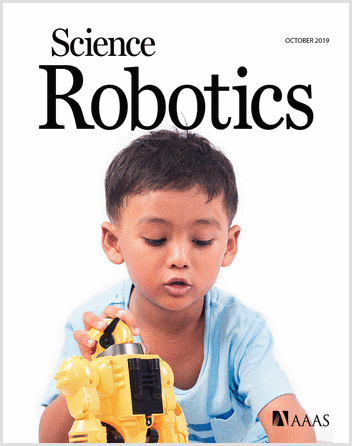
\includegraphics[height=2.2cm]{thumbs/2019-science.png} & Senft, E.,
    \ul{Lemaignan, S.}, Baxter, P., Bartlett, M., Belpaeme, T.
    \newline\href{https://doi.org/10.1126/scirobotics.aat1186}{\textbf{Teaching robots
    social autonomy from in situ human guidance}}
    \newline \textit{Science Robotics} 2019
    & \small A novel human-in-the-loop machine learning approach
    to implement social autonomy in a robot, with several deployments in UK
    public schools. This is a first-in-kind demonstration of learning autonomous
    action policy in a high dimensional, socially complex,
    environment.\textbf{\newline[main study supervisor]} \\


    \vspace{-.20cm}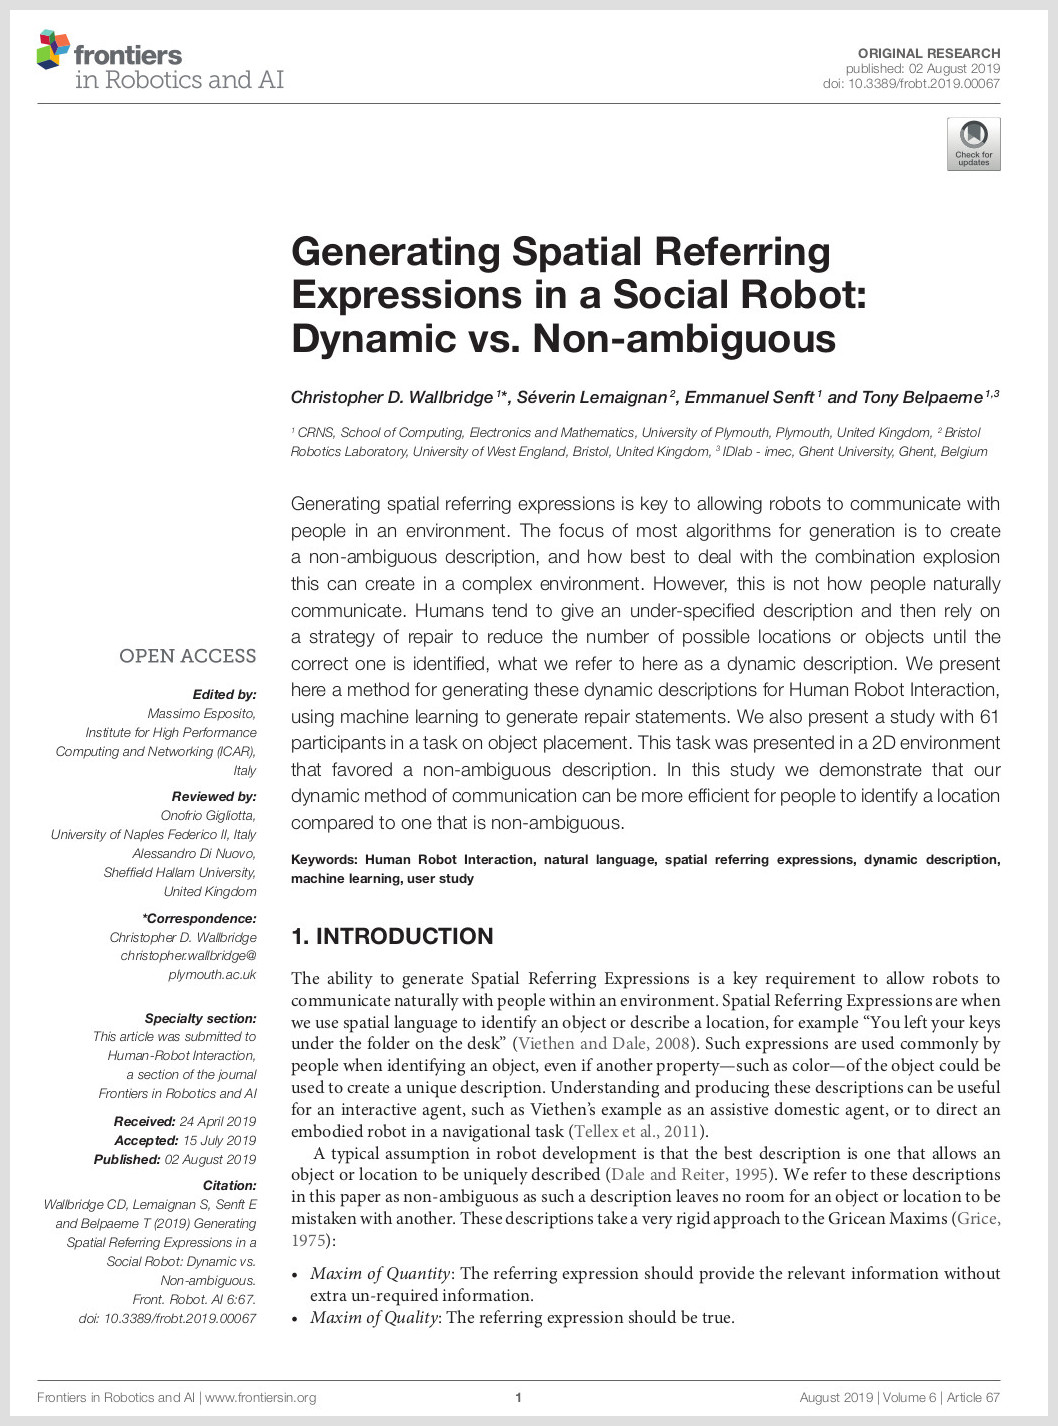
\includegraphics[height=2.2cm]{thumbs/2019-frontiers-chris.jpg} &

    Wallbridge, C., \ul{Lemaignan, S.}, Senft, E., Belpaeme, T.  
    \newline\href{https://doi.org/10.3389/frobt.2019.00067}{\textbf{Generating
    Spatial Referring Expressions in a Social Robot: Dynamic vs Non-Ambiguous}}
    \newline \textit{Frontiers in AI and Robotics} 2019
    & \small Challenges the common understanding that robots should be
    unambiguous: we show that ambiguity is often desirable for fluid and natural
    human-robot interactions.\textbf{\newline[main study supervisor]}  \\

    \vspace{-.20cm}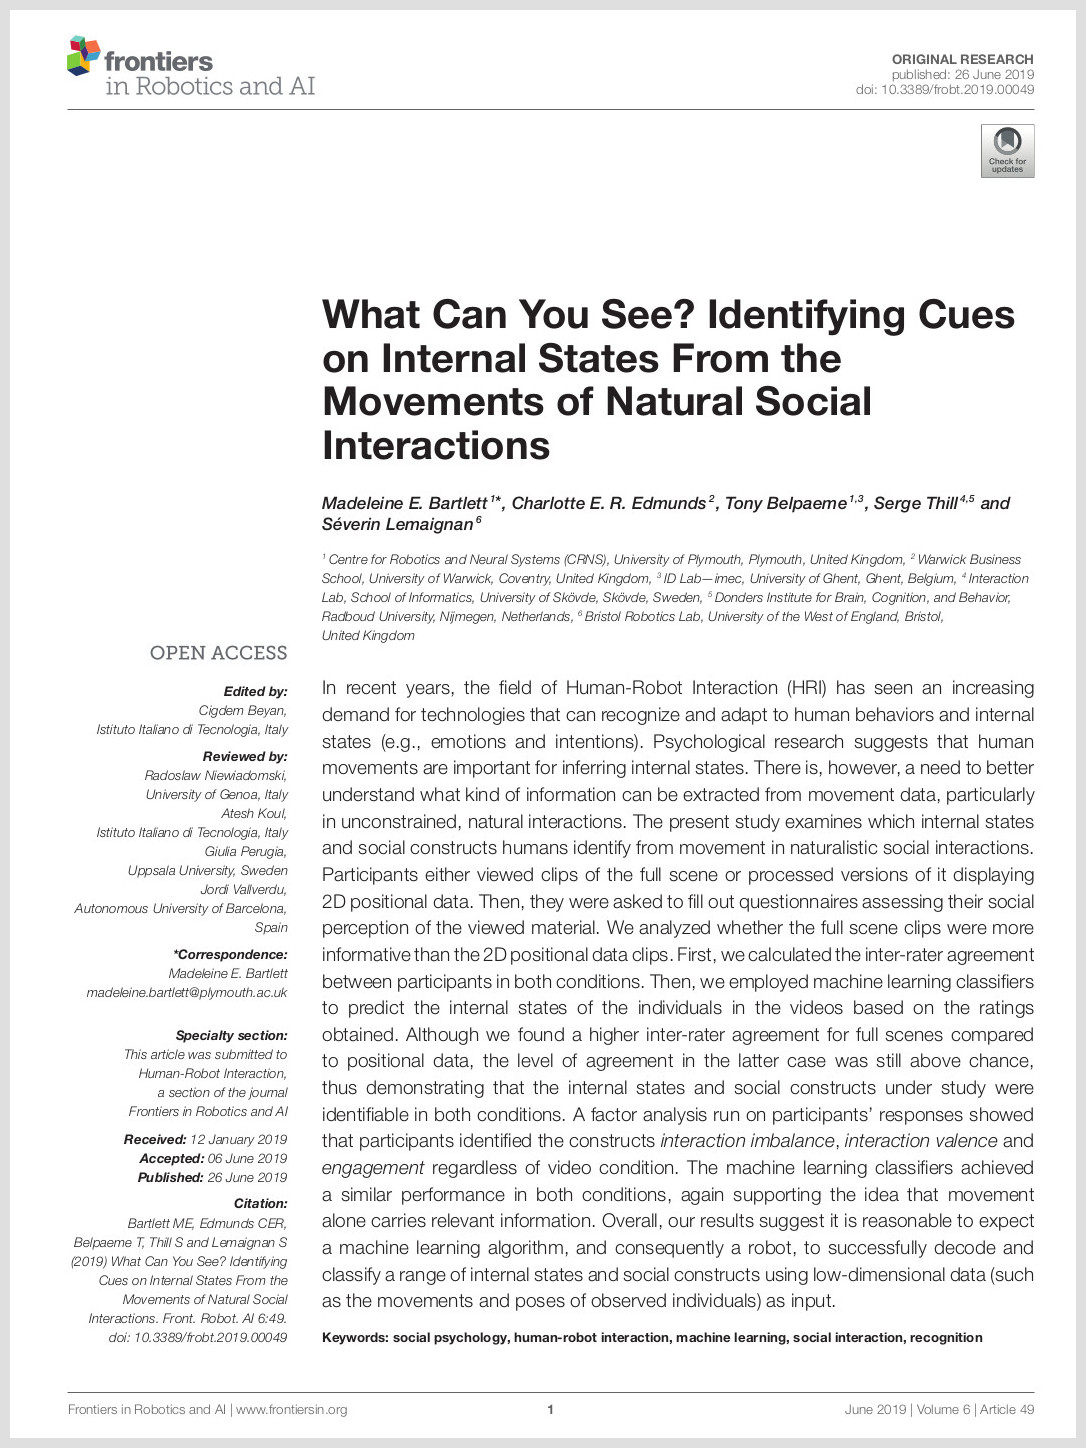
\includegraphics[height=2.2cm]{thumbs/2019-frontiers-maddy.jpg} &

    Bartlett, M., Edmunds, C. E. R., Belpaeme, T., Thill, S., \ul{Lemaignan, S.} 
    \href{https://doi.org/10.3389/frobt.2019.00049}{\textbf{What Can You See? Identifying Cues on Internal States from the
    Kinematics of Natural Social Interactions}} 
    \newline \textit{Frontiers in AI and Robotics} 2019
    & \small Investigates how partially hidden `internal states' (like emotions,
    cooperativeness, etc) can be decoded from simple visible cues, like
    skeletons. Also demonstrates that social situations can be described along 3
    simple dimensions.\textbf{\newline[main study supervisor]}\\


    \vspace{-.20cm}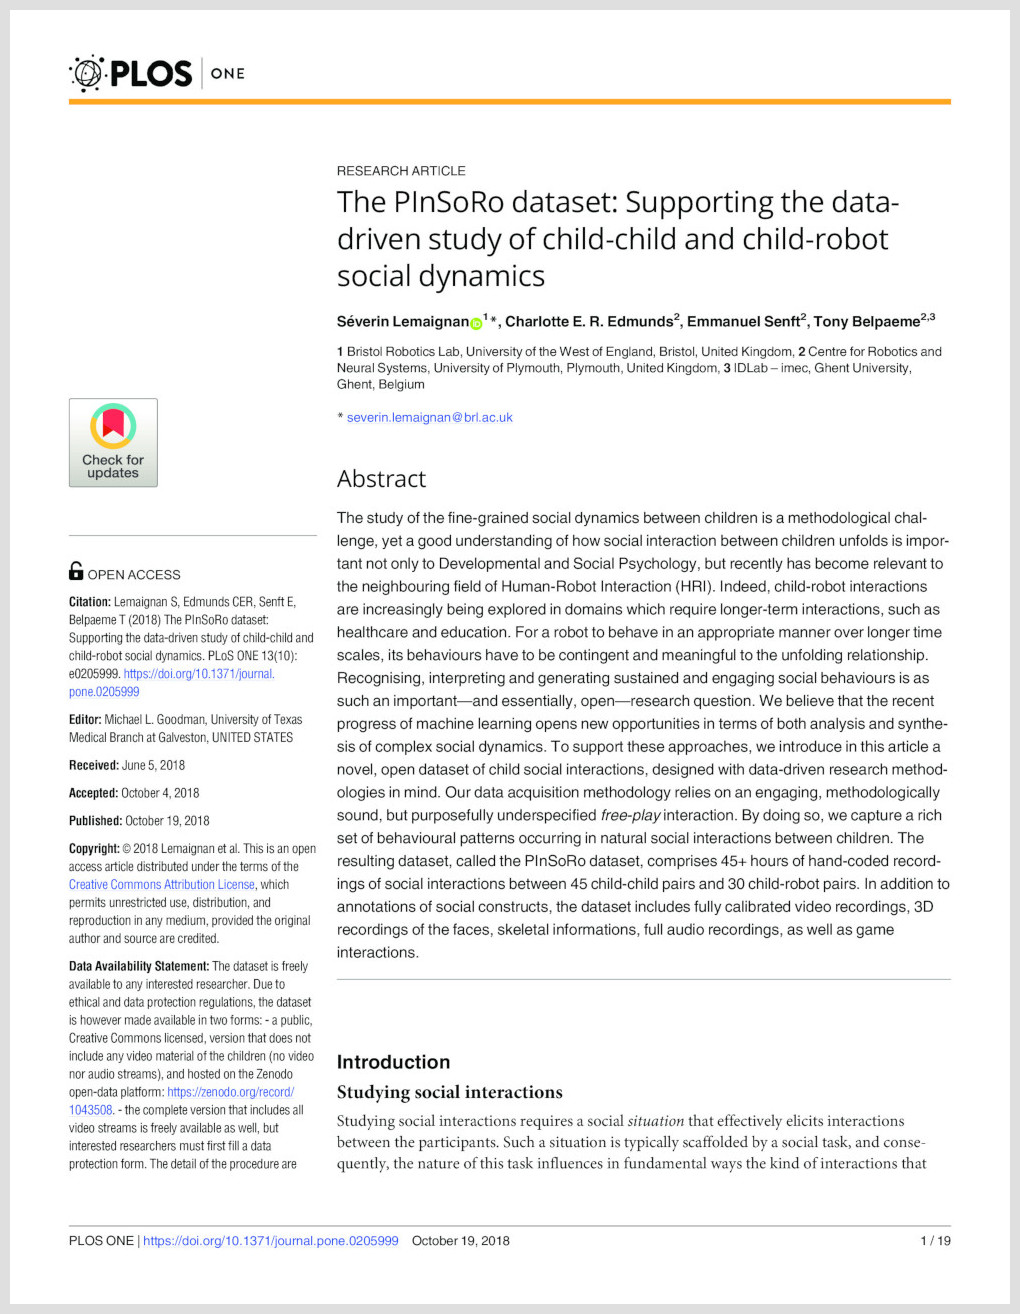
\includegraphics[height=2.2cm]{thumbs/2018-plosone.jpg} &

    \ul{Lemaignan, S.}, Edmunds E. R., C., Senft, E., Belpaeme, T.
    \newline\href{https://doi.org/10.1371/journal.pone.0205999}{\textbf{The
    PInSoRo dataset: Supporting the data-driven study of child-robot social
    dynamics}}
    \newline \textit{PLOS ONE} 2018
    & \small A first-in-kind, large scale dataset of child-child and child-robot social interactions. Design
    with machine learning in mind, this dataset effectively opens up the field
    of data-driven social psychology, with direct applications in AI and social
    robotics.\textbf{[principal investigator]}\\

    \vspace{-.20cm}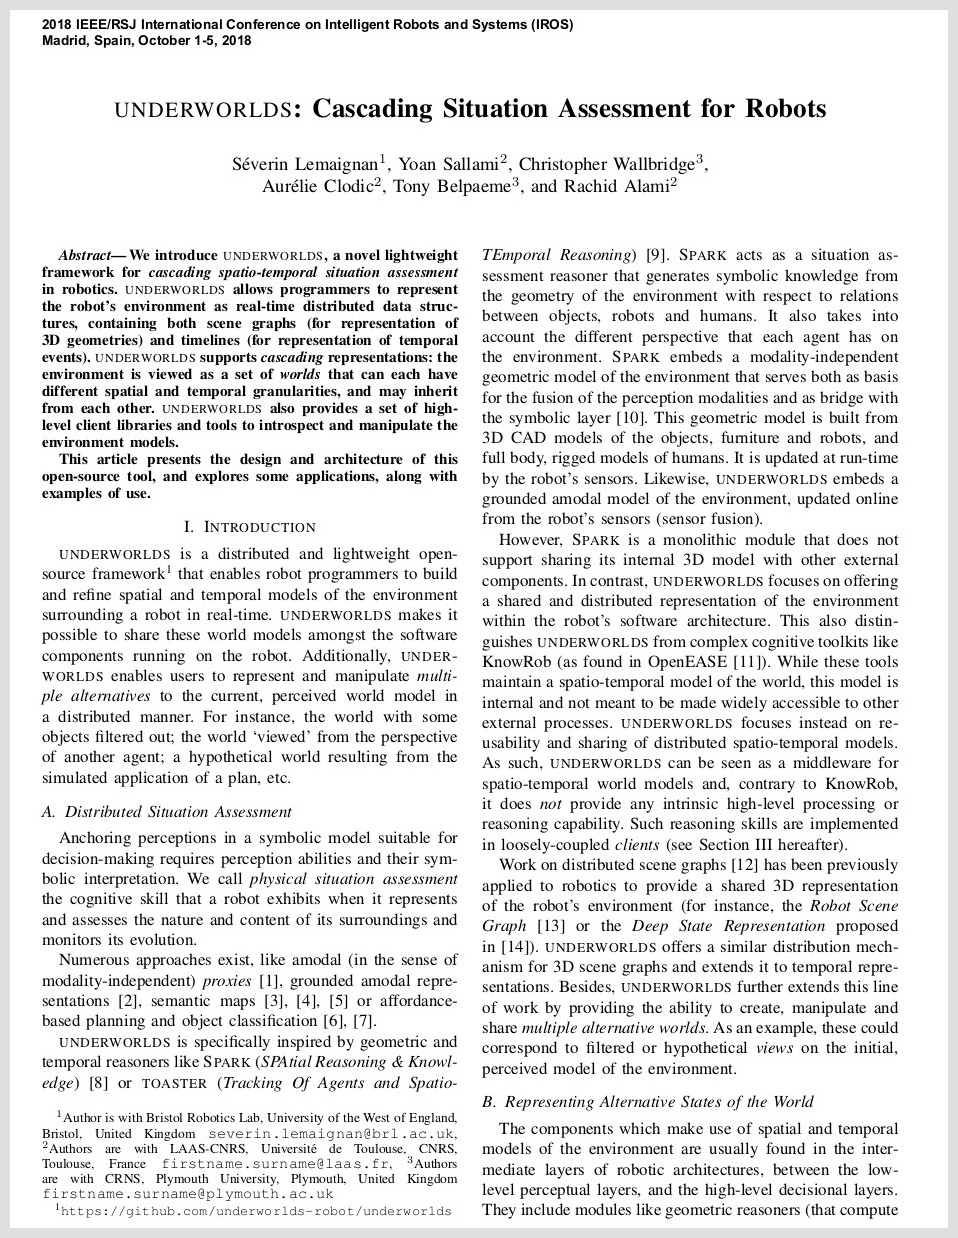
\includegraphics[height=2.2cm]{thumbs/2018-underworlds.jpg} &

    \ul{Lemaignan, S.}, Sallami, Y., Wallbridge, C., Clodic, A., Alami,
    R. 
   \newline\href{https://doi.org/10.1109/IROS.2018.8594094}{\textbf{\sc
    underworlds: Cascading Situation Assessment for Robots}}
    \newline\textit{IEEE IROS} 2018

    & \small A novel representation technique to efficiently
    represent multiple parallel states of the world, including imaginary ones.
    This ability is critical to represent spatio-temporal predictions, and to
    create models of other agents' representations.
    \textbf{[principal investigator]}\\



    \vspace{-.20cm}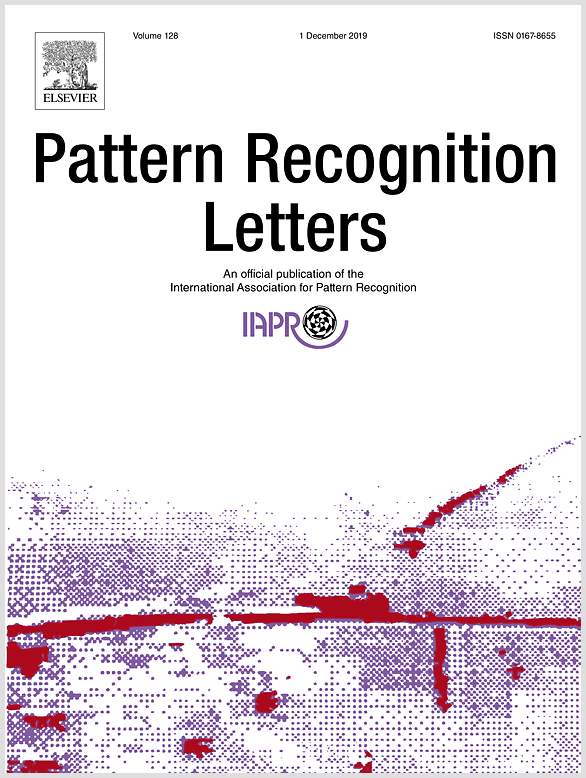
\includegraphics[height=2.2cm]{thumbs/2017-sparc.jpg} &

    Senft, E., Baxter, P., Kennedy, J., \ul{Lemaignan, S.}, Belpaeme, T.
    \newline\href{https://doi.org/10.1016/j.patrec.2017.03.015}{\textbf{Supervised
    Autonomy for Online Learning in Human-Robot Interaction}}
    \newline \textit{Pattern Recognition Letters} 2017
    & \small The mathematical and technical bases of the SPARC
    paradigm for human-in-the-loop machine learning, showing that
    high-dimensional problems can be learnt effectively and rapidely thanks to
    an innovative input feature selection mechanism.
    \textbf{\newline[student supervisor; 22 citations]}\\


    \vspace{-.20cm}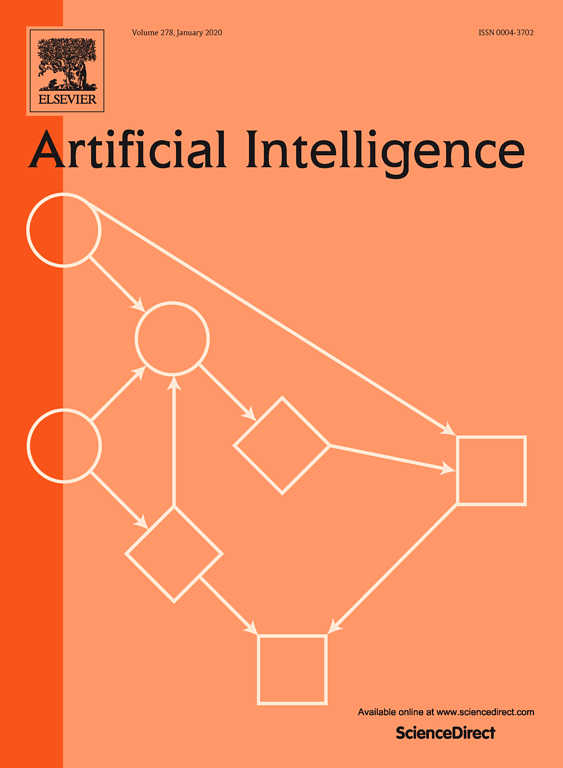
\includegraphics[height=2.2cm]{thumbs/2017-ai-cover.jpg} &

    \ul{Lemaignan, S.}, Warnier, M., Sisbot, E.A., Clodic, A., Alami, R.
    \newline
    \href{https://doi.org/10.1016/j.artint.2016.07.002}{\textbf{Artificial
    Cognition for Social Human-Robot Interaction: An Implementation}}
    \newline \textit{Artificial Intelligence} 2017
    & \small Landmark article: one of the first complete, semantic-aware, robotic architecture for
    human-robot interaction, including symbolic knowledge representation,
    situation assessment, natural language grounding, task planning, human-aware
    motion planning and execution. \textbf{\newline[principal investigator and
    coordinator; 143 citations]}\\

\end{tabular}

\hspace*{-0.5cm}\begin{tabular}{p{1.7cm}p{7cm}p{8cm}}


    \vspace{-.20cm}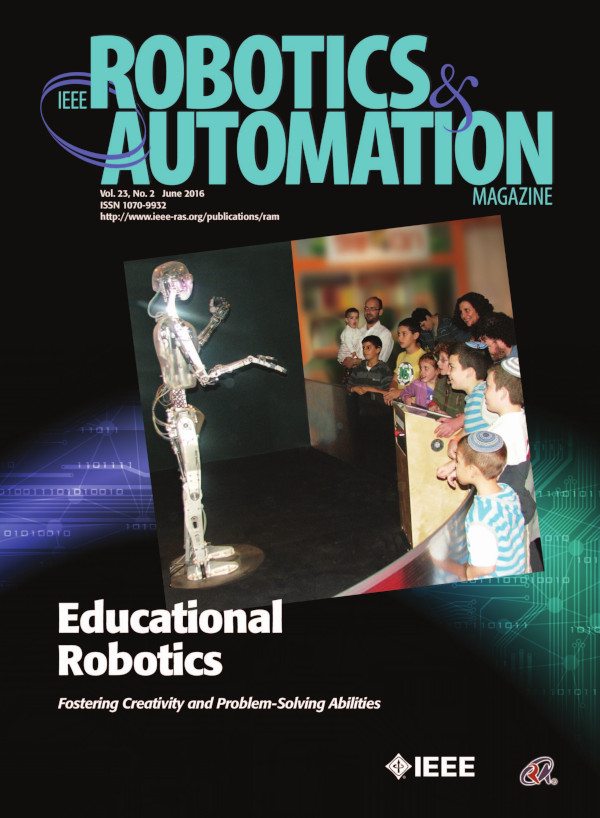
\includegraphics[height=2.2cm]{thumbs/2016-cowriter.jpg} &

    \ul{Lemaignan, S.}, Jacq, A., Hood, D., Garcia, F., Paiva, A., Dillenbourg, P.
    \newline
    \href{https://doi.org/10.1109/MRA.2016.2546700}{\textbf{Learning by
    Teaching a Robot: The Case of Handwriting}}
    \newline \textit{Robotics and Automation Magazine} 2016
    & \small Long-term studies with children and
    therapists, where we \emph{reverse} the social role of the
    robot to significantly improve the children' self-confidence. A landmark in
    social robotics for education. \textbf{\newline[principal investigator; 141
    citations} (incl. conf. article) \textbf{]}\\



    \vspace{-.20cm}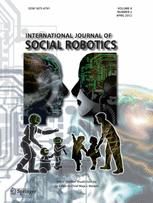
\includegraphics[height=2.2cm]{thumbs/2012-grounding.jpg} &

    \ul{Lemaignan, S.}, Ros, R., Sisbot, E. A., Alami, R., Beetz M.
    \href{https://doi.org/10.1007/s12369-011-0123-x}{\textbf{Grounding
    the Interaction: Anchoring Situated Discourse in Everyday Human-Robot
    Interaction}} 
    \newline \textit{Intl Journal of Social Robotics} 2012

    & \small In this paper, I show how symbolic knowledge representation can be
    used by robot to ground natural language interactions, also taking into
    account the unique perspective of the human interactor.
    \textbf{\newline[principal investigator; 100 citations]}\\

    \vspace{-.20cm}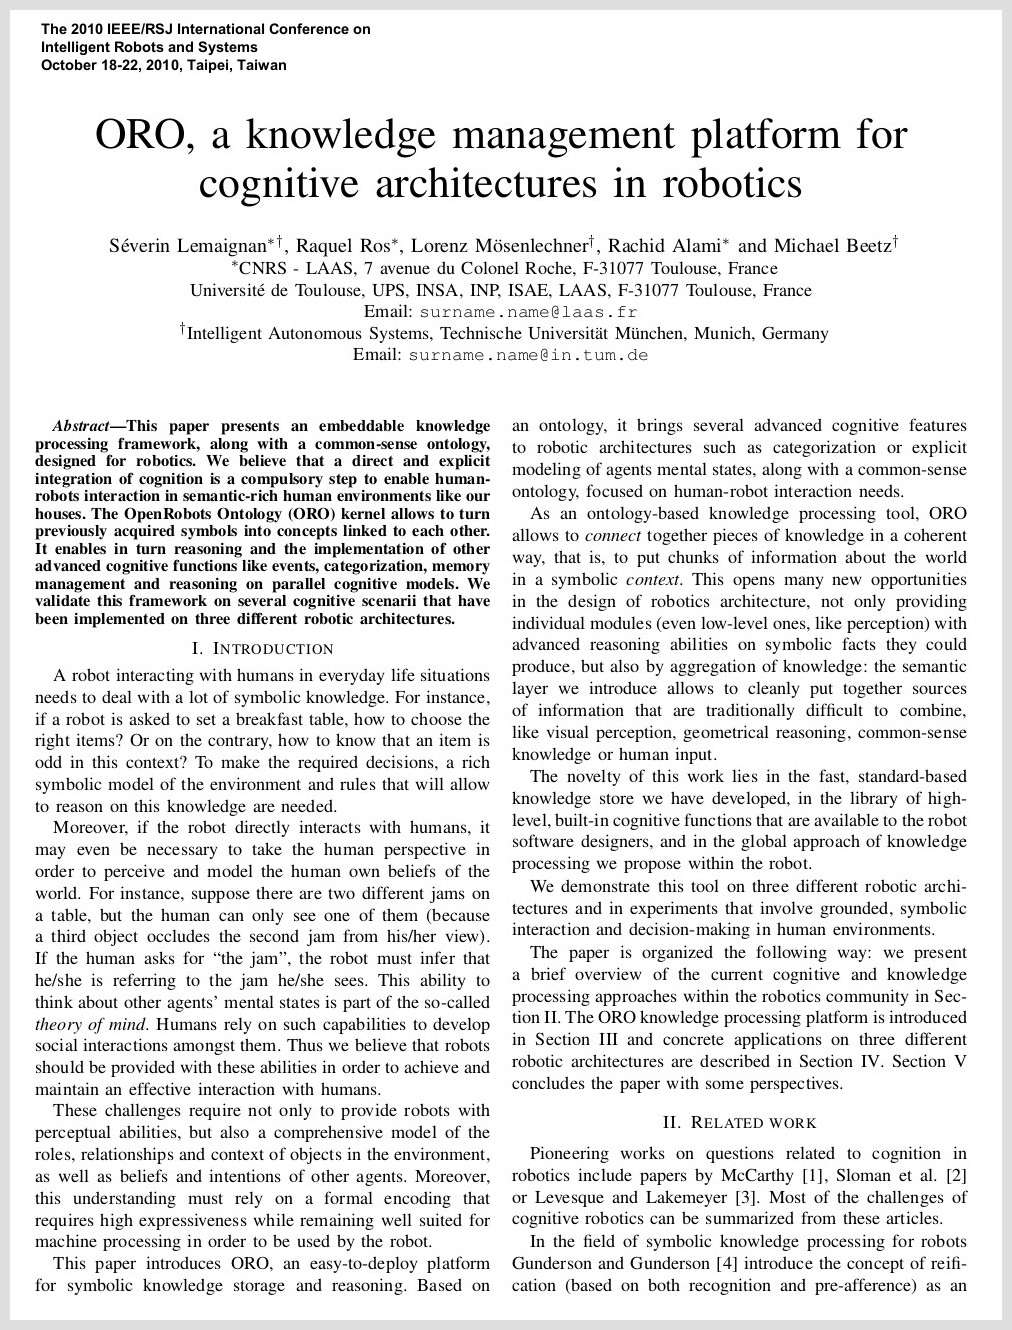
\includegraphics[height=2.2cm]{thumbs/2010-oro.jpg} &
    \ul{Lemaignan, S.}, Ros, R., Mösenlechner, L., Alami, R., Beetz, M.
    \newline\href{https://doi.org/10.1109/IROS.2010.5649547}{\textbf{ORO, a Knowledge Management Module for Cognitive Architectures in
    Robotics}}
    \newline \textit{IEEE IROS} 2010

    & \small One of the very first knowledge base designed and
    integrated in service robots. Pioneering work which played a key role in
    understanding how intelligent robot can represent their
    knowledge to facilitate communication with humans.
    \textbf{\newline[principal investigator; 158 citations]}\\

\end{tabular}


\subsection{Fellowships and awards}

\begin{tabular}{p{0.15\linewidth}p{0.8\linewidth}}
    \bf 2019 & UWE Vice Chancellor Accelerator Fellowship \\
    \bf 2015 -- 2017 & {\bf EU Marie Skłodowska-Curie Individual Fellowship}
    \newline Theory of Mind and social robotics, Plymouth University, UK \\
    \bf HRI'2017  & Best Paper award\\
    \bf HRI'2016  & Best Paper award\\
    \bf AAAI'2015  & Best Video award in Artificial Intelligence\\
    \bf HRI'2014  & Best Late Breaking Report award\\
    \bf 2012         & {\bf Best PhD in Robotics 2012} award, CNRS, France \\
    \bf 2012         & PhD with {\bf High Distinction} (“Summa Cum Laude”), TU Munich\\
    \bf Ro-Man'2010  & Best paper award\\
\end{tabular}

\vspace{2em}
\section{Contributions to the development of individuals}

Since 2018, I co-supervise the BRL's \emph{Human-Robot Interaction} (15 people) and \emph{Driverless Vehicles} (5 people) research groups.
I directly line-manage 4 students and early career researchers.\\

\subsection{Supervision of graduate students and postdoctoral fellows}

\begin{tabular}{p{0.15\linewidth}p{0.8\linewidth}}
    \bf 2018 -- 2019 & \textbf{2 post-docs}, \textbf{5 PhDs}, \textbf{4 MSc students}, Bristol Robotics Lab, UWE, UK \\
    \bf 2015 -- 2018 & \textbf{3 PhDs}, Plymouth University, UK \\
    \bf 2013 -- 2015 & \textbf{5 PhDs}, \textbf{5 MSc students}, EPFL, Switzerland \\
    \bf 2012 -- 2013 & \textbf{2 MSc students}, LAAS-CNRS, France \\
\end{tabular}


\subsection{Teaching activities}

\begin{tabular}{p{0.15\linewidth}p{0.8\linewidth}}
    \bf 2019 --  & \textbf{Associate Professor} teaching at postgraduate level, UWE, UK \\
    \bf 2018 -- 2019 & \textbf{Senior Lecturer} teaching at postgraduate level, UWE, UK \\
    \bf 2015 -- 2018 & \textbf{Lecturer} teaching at undergraduate \&
    postgraduate levels (robotics fundamentals, software engineering, human-robot interaction), Plymouth University, UK \\
    \bf 2013 -- 2015 & \textbf{Teaching Assistant} teaching at undergraduate level (Visual Computing), EPFL, Switzerland \\
    \bf 2008 -- 2012 & \textbf{Teaching Assistant} teaching at undergraduate level (programming, databases, ontologies), INSA Toulouse, France \\
\end{tabular}

\vspace{2em}
\section{Contributions to the wider research community}
\subsection{Organisation of scientific meetings}

\begin{tabular}{p{0.05\linewidth}p{0.9\linewidth}}
    \bf 2020 & \textbf{ACM/IEEE Human-Robot Interaction conference}, 700+ participants, local chair, Cambridge, UK \\
    \bf 2017 & \textbf{ACM/IEEE Human-Robot Interaction conference}, 400+
    participants, alt.HRI chair, Vienna, AT \\
    \bf 2016 & \textbf{2nd Intl. workshop on Cognitive Architecture for Social HRI}, 45 participants, programme chair, Christchurch, NZ \\
    \bf 2014 & \textbf{Intl. workshop on Simulation for HRI}, 35 participants, programme chair, Bielefeld, DE \\
    \bf 2012 & \textbf{Intl. workshop on MORSE and its applications}, 30 participants, programme chair, Toulouse, FR \\
    \bf 2009 & \textbf{Cognitive Sciences’ Young Researchers Conference}, 150 participants, steering committee, Toulouse, FR \\
\end{tabular}

\subsection{Institutional responsibilities}

\begin{tabular}{p{0.15\linewidth}p{0.8\linewidth}}
    \bf 2019 -- & Full member of the EPSRC Peer Review college \\
    \bf 2019 -- & Head of the Outreach cluster, Faculty of Technology and Environment, UWE, UK \\
    \bf 2019 & PhD defense committee, University of Bielefeld, DE \\
    \bf 2019 & PhD defense committee, University of Örebro, SE \\
    \bf 2018 -- & HRI module co-lead, MSc level, University of the West of England, UK  \\
    \bf 2017 -- 2018 & Module leader, Robotics fundamentals (undergraduate level), University of Plymouth, UK \\
\end{tabular}

\subsection{Editorial activities}

\begin{tabular}{p{0.15\linewidth}p{0.8\linewidth}}
    \bf 2019 --  & Member of the Robotics, Science and System (RSS) Programme Committee  \\
    \bf 2018 --  & Editorial board of \emph{Frontiers in AI and Robotics} \\
    \bf 2017 --  & Member of the IJCAI Programme Committee  \\
    \bf 2015 --  & Member of the IEEE/ACM HRI Programme Committee \\
    \bf 2017 -- 2019 & Member of the IEEE IROS Programme Committee  \\
    \bf 2017 -- 2018 & Member of the HAI Programme Committee  \\
\end{tabular}

\vspace{2em}
\section{Contributions to the broader society}

\subsection{Policy making}

\begin{tabular}{p{0.15\linewidth}p{0.8\linewidth}}
    \bf 2020 -- & {\bf Expert Collaborator for the European Joint Research Centre} contributing to the UNICEF Guidelines for Responsible Child-Robots Interactions \\
    \bf 2019  & {\bf Invited panel by the EU Research Executive Agency} at the 2019 MSCA AI Cluster, sharing expertise in Human-Robot Interaction \\
\end{tabular}

\subsection{Technology transfer}
\begin{tabular}{p{0.15\linewidth}p{0.8\linewidth}}
    \bf 2018 -- & Co-I on UKRI InnovateUK projects ROBOPILOT, CAPRI, CAVForth, involving direct transfer of technology for automated verification of autonomous vehicles \\
    \bf 2018 -- & Scientific advisor for KickSum Ltd., in the frame of the EU-funded SABRE project \\
    \bf 2018  & Co-inventor on US patent US20190016213A1 on back-driveable, haptic locomotion for small robots \\
\end{tabular}

\subsection{Outreach and public dissemination}
\begin{tabular}{p{0.15\linewidth}p{0.8\linewidth}}
    \bf 2018 --  & Technology transfer: Member of the Robotics, Science and System (RSS) Programme Committee  \\
\end{tabular}


\vspace{2em}



%\section{MAJOR COLLABORATIONS}

%Name of collaborators, Topic, Name of Faculty/ Department/Centre, Name of University/ Institution/ Country

%%%%%%%%%%%%%%%%%%%%%%%%%%%%%%%%%%%%%%%%%%%%%%%%%%%%%%%%%%%%%%%%%%%%%%%%%%%%%%%%%%%%%%%%%%%%%%%%%%%%%%%%%%%%
%\section{}

%%%%%%%%%%%%%%%%%%%%%%%%%%%%%%%%%%%%%%%%%%%%%%%%%%%%%%%%%%%%%%%%%%%%%%%%%%%%%%%%%%%%%%%%%%%%%%%%%%%%%%%%%%%%
%\section{}

%%%%%%%%%%%%%%%%%%%%%%%%%%%%%%%%%%%%%%%%%%%%%%%%%%%%%%%%%%%%%%%%%%%%%%%%%%%%%%%%%%%%%%%%%%%%%%%%%%%%%%%%%%%%
%\section{}

